%% Creator: Inkscape inkscape 0.48.4, www.inkscape.org
%% PDF/EPS/PS + LaTeX output extension by Johan Engelen, 2010
%% Accompanies image file 'pb_opt_iga.pdf' (pdf, eps, ps)
%%
%% To include the image in your LaTeX document, write
%%   \input{<filename>.pdf_tex}
%%  instead of
%%   \includegraphics{<filename>.pdf}
%% To scale the image, write
%%   \def\svgwidth{<desired width>}
%%   \input{<filename>.pdf_tex}
%%  instead of
%%   \includegraphics[width=<desired width>]{<filename>.pdf}
%%
%% Images with a different path to the parent latex file can
%% be accessed with the `import' package (which may need to be
%% installed) using
%%   \usepackage{import}
%% in the preamble, and then including the image with
%%   \import{<path to file>}{<filename>.pdf_tex}
%% Alternatively, one can specify
%%   \graphicspath{{<path to file>/}}
%%
%% For more information, please see info/svg-inkscape on CTAN:
%%   http://tug.ctan.org/tex-archive/info/svg-inkscape
%%
\begingroup%
  \makeatletter%
  \providecommand\color[2][]{%
    \errmessage{(Inkscape) Color is used for the text in Inkscape, but the package 'color.sty' is not loaded}%
    \renewcommand\color[2][]{}%
  }%
  \providecommand\transparent[1]{%
    \errmessage{(Inkscape) Transparency is used (non-zero) for the text in Inkscape, but the package 'transparent.sty' is not loaded}%
    \renewcommand\transparent[1]{}%
  }%
  \providecommand\rotatebox[2]{#2}%
  \ifx\svgwidth\undefined%
    \setlength{\unitlength}{500bp}%
    \ifx\svgscale\undefined%
      \relax%
    \else%
      \setlength{\unitlength}{\unitlength * \real{\svgscale}}%
    \fi%
  \else%
    \setlength{\unitlength}{\svgwidth}%
  \fi%
  \global\let\svgwidth\undefined%
  \global\let\svgscale\undefined%
  \makeatother%
  \begin{picture}(1,0.24)%
    \put(0,0){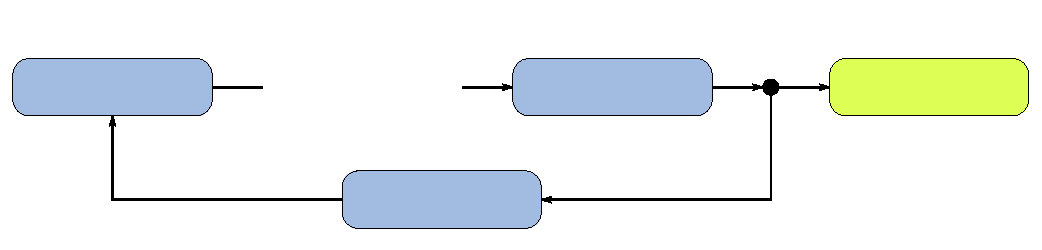
\includegraphics[width=\unitlength]{figures/pb_opt_iga.pdf}}%
    \put(0.34736877,0.15257358){\color[rgb]{0,0,0}\makebox(0,0)[b]{\smash{\large \textbf{\faSmileO~Refinement}}}}%
    \put(0.10835595,0.15959788){\color[rgb]{0,0,0}\makebox(0,0)[b]{\smash{CAD Model}}}%
    \put(0.10768077,0.13785865){\color[rgb]{0,0,0}\makebox(0,0)[b]{\smash{generation}}}%
    \put(0.58820565,0.14911261){\color[rgb]{0,0,0}\makebox(0,0)[b]{\smash{Simulation}}}%
    \put(0.76153551,0.16175593){\color[rgb]{0,0,0}\makebox(0,0)[b]{\smash{\footnotesize Yes}}}%
    \put(0.7226443,0.05406804){\color[rgb]{0,0,0}\makebox(0,0)[b]{\smash{\footnotesize No}}}%
    \put(0.4244494,0.05507856){\color[rgb]{0,0,0}\makebox(0,0)[b]{\smash{Optimization}}}%
    \put(0.42430879,0.0308687){\color[rgb]{0,0,0}\makebox(0,0)[b]{\smash{algorithm}}}%
    \put(0.8915822,0.15097365){\color[rgb]{0,0,0}\makebox(0,0)[b]{\smash{\textit{Optimal Design}}}}%
    %
    \put(0.05,0.225){\color[rgb]{0,0,0}\makebox(0,0)[b]{\Large\smash{\textbf{\texttt{IGA framework:}}}}}%
  \end{picture}%
\endgroup%
